\documentclass[11pt]{article}

\usepackage[margin=1in]{geometry}
\usepackage{tikz}
\usepackage{amsmath}
\usepackage{amssymb}

\begin{document}

\begin{flushright}
Andrew Leverentz
\end{flushright}

We begin by considering a taxonomy of hierarchical clustering algorithms (Figure \ref{fig:taxonomy}).
A \emph{hierarchical clustering} is a tree in which the leaves correspond to individual points in the input dataset, and each internal node corresponds to the subset of the data corresponding to the node's descendant leaves.
Then, a \emph{hierarchical clustering algorithm} is merely an algorithm which takes as input an unlabeled dataset and outputs a hierarchical clustering.
When constructing a hierarchical clustering, the goal is typically to find a nested set of splits which separate highly ``dissimilar'' points toward the top of the tree, and which separate highly ``similar'' points much closer to the leaves.

\begin{figure}[h]
\centering
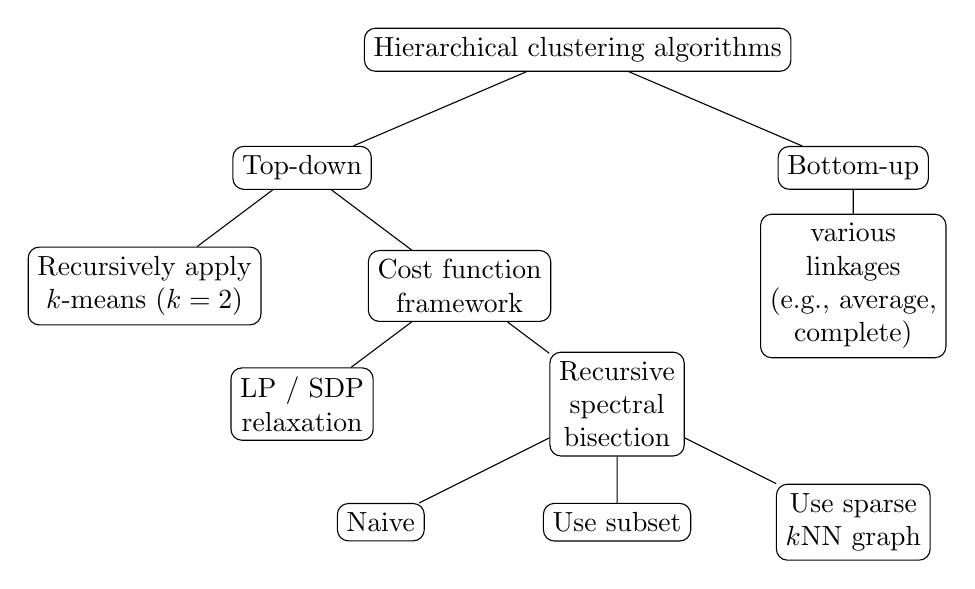
\begin{tikzpicture}[
  every node/.style = {
    shape=rectangle,
    rounded corners,
    draw,
    align=center
  },
  level 1/.style={sibling distance=7cm},
  level 2/.style={sibling distance=4cm},
  level 3/.style={sibling distance=4cm},
  level 4/.style={sibling distance=3cm},
  level 5/.style={sibling distance=3cm},]
  \node {Hierarchical clustering algorithms}
    child { node {Top-down}
      child { node {Recursively apply \\ $k$-means ($k = 2$)} }
      child { node {Cost function \\ framework}
        child { node {LP / SDP \\ relaxation} }
        child { node {Recursive \\ spectral \\ bisection}
          child { node {Naive} }
          child { node {Use subset} }
          child { node {Use sparse \\ $k$NN graph} }
        }
      }
    }
    child { node {Bottom-up}
      child { node {various \\ linkages \\ (e.g., average, \\ complete)}}
    };
\end{tikzpicture}
\caption{Taxonomy of hierarchical clustering algorithms}
\label{fig:taxonomy}
\end{figure}

A hierarchical clustering algorithm may be either bottom-up or top-down.
A \emph{bottom-up} algorithm starts by putting each observation into its own cluster, and it repeatedly combines them according to some criterion (e.g., single linkage, average linkage, and so on).
This approach is ``bottom-up'' because we start at the leaves and work our way toward the root by combining clusters.
A \emph{top-down} algorithm starts by putting all observations into a single cluster, and it repeatedly divides each node according to some criterion.
In this setting, we start at the root and work our way toward the leaves.

One approach to top-down clustering is to recursively apply a simple binary splitting algorithm (such as $k$-means with $k=2$).
However, one major downside to this approach is that it cannot handle clusters with highly irregular boundaries, and in such cases it may end up producing splits which place very similar points into different high-level clusters.

Dasgupta [2016] defines a cost-function framework for hierarchical clustering.
Any algorithm which minimizes (or approximately minimizes) the given cost function belongs to this class.
One particular subset of these algorithms are those which recursively split clusters into two, while attempting to minimize the RatioCut (**TODO: confirm terminology) at each stage.

Several authors (**TODO: citations) have proposed optimizing the via relaxations (LP or SDP).
Unfortunately, these algorithms have runtimes of $\Omega(n^3)$ and therefore suffer from the same scaling limitations as most bottom-up clustering algorithms.

Recursive spectral bisection (i.e., repeated application of 2-way spectral clustering) involves computing a particular eigenvector (the ``Fiedler vector'') of the graph Laplacian corresponding to the pairwise similarity matrix of the dataset.
This approach is known to approximately minimize the RatioCut (**TODO: confirm terminology) of the similarity graph.
However, a naive implentation, using a dense similarity matrix and standard eigenvector computations, once again has a runtime of $\Omega(n^3)$.

Several modifications to recursive spectral bisection can improve its performance:
\begin{enumerate}
    \item Applying spectral clustering to the result of $k$-means clustering (where $k \ll n$)
    \item Using a randomly selected subset
    \item Constructing a sparse $k$-nearest neighbor ($k$NN) graph prior to performing spectral clustering
\end{enumerate}

For now, we focus on the third option. 
Using Fast Nearest Neighbor data structures (such as metric trees or random projection trees), we can efficiently compute a sparse $k$NN graph.
From this sparse $k$NN graph, we construct a sparse similarity matrix and then apply spectral clustering.

There are several important considerations involved in this process:
\begin{itemize}
    \item Converting a distance matrix to a similarity matrix involves a scaling parameter which needs to be selected according to an adaptive criterion.
    \item The parameter $k$ should grow as a function of $n$ (otherwise the sparse similarity graph will contain a large number of disconnected components), but if it grows too quickly, the algorithm will no longer scale sub-quadratically.  (Ideally, $k$ should be sublinear in the dataset size $n$; for example, $k \in O(\log n)$.)
    \item The algorithm should handle disconnected components in a sensible way (for example, by partitioning them such that the number of observations assigned to each side of a split is roughly balanced).
    \item Linear algebra operations (in particular, eigenvalue/eigenvector computations) must be implemented in a way that takes advantage of the sparsity of the similarity matrix.
\end{itemize}

\end{document}